\section{Kodo skirstymo į paketus šablonų analizė}
Atviro kodo analizės metu buvo išskirti septyni kodo skirstymo į paketus šablonai.
Norint įvertinti, kuris šablonas duotai problemai spręsti yra tinkamiausias, reikalinga nagrinėti, kaip siūlomas sprendimas
sprendžia atitinkamą problemą ir kokias pasekmes gali turėti jo taikymas.

\subsubsection{Pagalbinių, daugkartinio naudojimo klasių skirstymo šablonų analizė}
Pagalbinių klasių skirstymui buvo išskirti du šablonai - kiekvienai esybei priskirtos pagalbinės klasės bei atskiras pagalbinių klasių paketas.
Svarbi problema, susijusi su pagalbinėmis klasėmis - su sistema dirbantys inžinieriai nežino apie jų egzistavimą, todėl jų nenaudoja,
tai veda prie didesnio kodo pasikartojimo arba kelių skirtingų to paties pagalbinio funkcionalumo įgyvendinimų~\cite{Utility}.
Šią problemą sprendžia atskiras pagalbinių klasių paketas - naudojant tokį šabloną, programuotojas, susiduriantis su bendrine problema, kuri, tikėtina, jau yra išspręsta sistemoje, turėtų
aiškų procesą, kaip elgtis šioje situacijoje:
\begin{enumerate}
    \item Atsidaryti vieną paketą, skirtą pagalbinėms, daugkartinio naudojimo klasėms
    \item Pakete surasti klasę, kurios pavadinimas būtų susijęs su jo problema
    \item Klasės funkcijų saraše surasti jam tinkamą funkciją.
    \item Jei reikalingas funkcionalumas nerastas, įgyvendinti jį pasirinktoje klasėje.
    \item Iškviesti rastą arba sukurtą funkciją iš bendrinio panaudojimo kodo paketo savo funkcionalume
\end{enumerate}
Pakete reikėtų turėti atskiras klases kiekvienai bendrinei dalykinei sričiai, iš kurios pavadinimo programuotojas galėtų nuspresti,
kad jo ieškomas funkcionalumas bus būtent toje klasėje.
Tokį skirstymo būdą siūlo ir \textit{Domain-Driven Design: Tackling Complexity in the Heart of Software} autorius - šiuo atveju
pagalbinių klasių paketas galėtų būti laikomas palaikymui skirta dalykinės srities esybe.
Tokiu atveju svarbu užtikrinti, kad iš klasių pavadinimo aišku, kokią smulkesnę dalykinės srities sritį padengia klasė, bei kad šios klasės
neturėtų priklausomybių nuo jas naudojančių klasių - kitu atveju sudaromos ciklinės priklausomybės.

Skirstant pagalbines klases po ją naudojančios dalykinės srities esybės paketais, kyla kodo pasikartojimo rizika - nepatikrinus skirtingoms esybėms skirtų pagalbinių
klasių, sunku žinoti, ar toks funkcionalumas jau buvo įgyvendintas.
Išanalizavus galimus kodo skirstymo į paketus šablonus pagalbinių klasių skirstymui, galima teigti, kad tinkamesnis sprendimas šiai
problemai yra atskiras pagalbinių klasių paketas.

\subsubsection{Didelio klasių skaičius pakete skirstymo šablonų analizė}
Dideliam klasių pakete skaičiui spręsti buvo išskirti du šablonai - žemesnio lygio paketų sudarymas grupuojant pagal techninį sluoksnį ir
skirstymas pagal smulkų funkcionalumą.
Klasių skirstymas į paketus pagal techninį funkcionalumą dažnu atveju yra mažiau pastangų reikalaujantis metodas - atskirti,
pavyzdžiui, kurios klasės priklauso \textit{service} sluoksniui yra paprasčiau, nei įvertinti, kurių klasių teikiamas funkcionalumas yra glaudžiau susijęs.
Tačiau šis būdas ne taip efektyviai prisideda prie lengviau suprantamos sistemos struktūros -
hibridinis skirstymo metodas nesuteikia pilnos informacijos nei apie dalykinės srities esybes, nei apie technines sistemos dalis.
Taip pat, taikant šį metodą, gali kilti papildomų problemų - ne visas klases galima užtikrintai priskirti vienam sluoksniui.
Tokiu atveju, pavyzdžiui, esybės pagalbinėms klasėms, \textit{orchestrator} tipo klasėms reikėtų kurti papildomus paketus.

Skirstymą pagal smulkų funkcionalumą pagrindžia Robert C. Martin bendro sąryšio principas, kuris teigia, kad visos tarpusavyje susijusios klasės turėtų būti viename pakete ir
akcentuoja siekiamybę turėti gan mažus paketus, turinčius aiškiai apibrėžtą funkcionalumą, priežastį egzistuoti, taip užtikrinant ir
glaudų tarpusavyje susijusių klasių sąryšį.
Šis principas taip pat gali padėti sumažinti aferentinių jungčių skaičių paketuose.
Didelis priklausomybių nuo specifinio paketo skaičius (arba aferentinės jungtys), reiškia, kad pokyčiai tame pakete turės įtaką kelioms klasėms.
Funkcionalumas kitiems paketams galėtų būti pasiekiamas per vieną minimalią sąsają \angl{interface},
kuri atskleidžia tik konceptus (metodus arba duomenų tipus), kurie yra glaudžiai susiję su komponento teikiama paslauga, bei
klase, grąžinančią minėtos sąsajos įgyvendinimą.
Paketas, turintis vieną funkciją, yra naudojamas tik tų paketų, kuriems reikia būtent tos funkcijos,
taip užtikrinant tik mažos sistemos dalies priklausomybę nuo vieno paketo.
Taip pat mažas paketo funkcionalumas reiškia, kad minėtas paketas skirtas funkcionalumui įgyvendinti naudos minimalų kitų sistemos esybių skaičių,
taip sumažinant ir eferentinių jungčių skaičių.

Žemiau esančiuose paveikslėliuose galima matyti, kaip išskaidant paketus, turinčius kelis funkcionalumus (pavyzdys~\ref{img:excesive_deps}), yra sumažinamas paketų
priklausomybių skaičius (pavyzdys~\ref{img:good_deps}).
\begin{figure}[H]
    \centering
    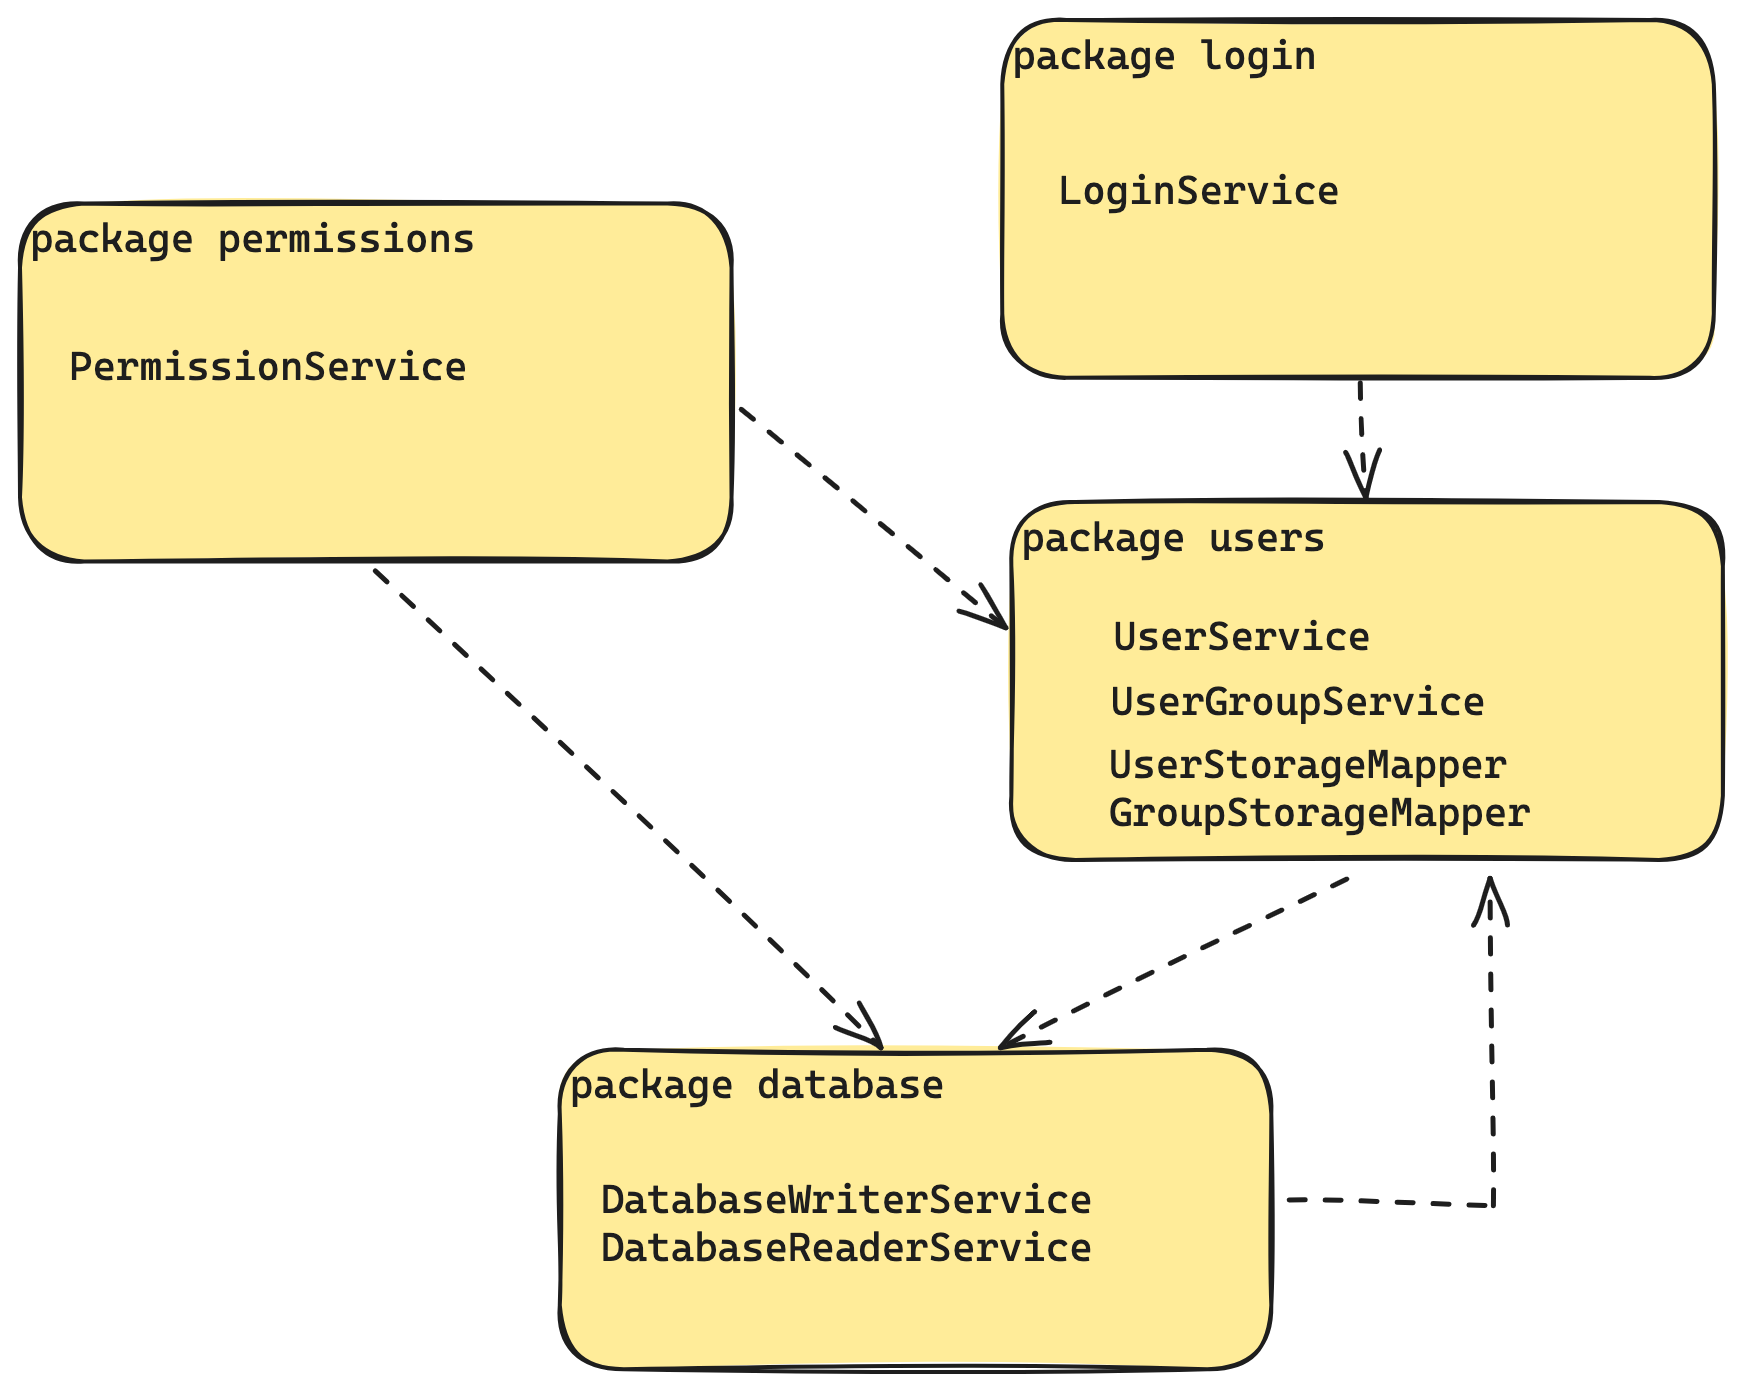
\includegraphics[scale=0.15]{img/excesive_deps}
    \caption{Sistemos pavyzdys su kelias funkcijas atliekančiais paketais}
    \label{img:excesive_deps}
\end{figure}


\begin{figure}[H]
    \centering
    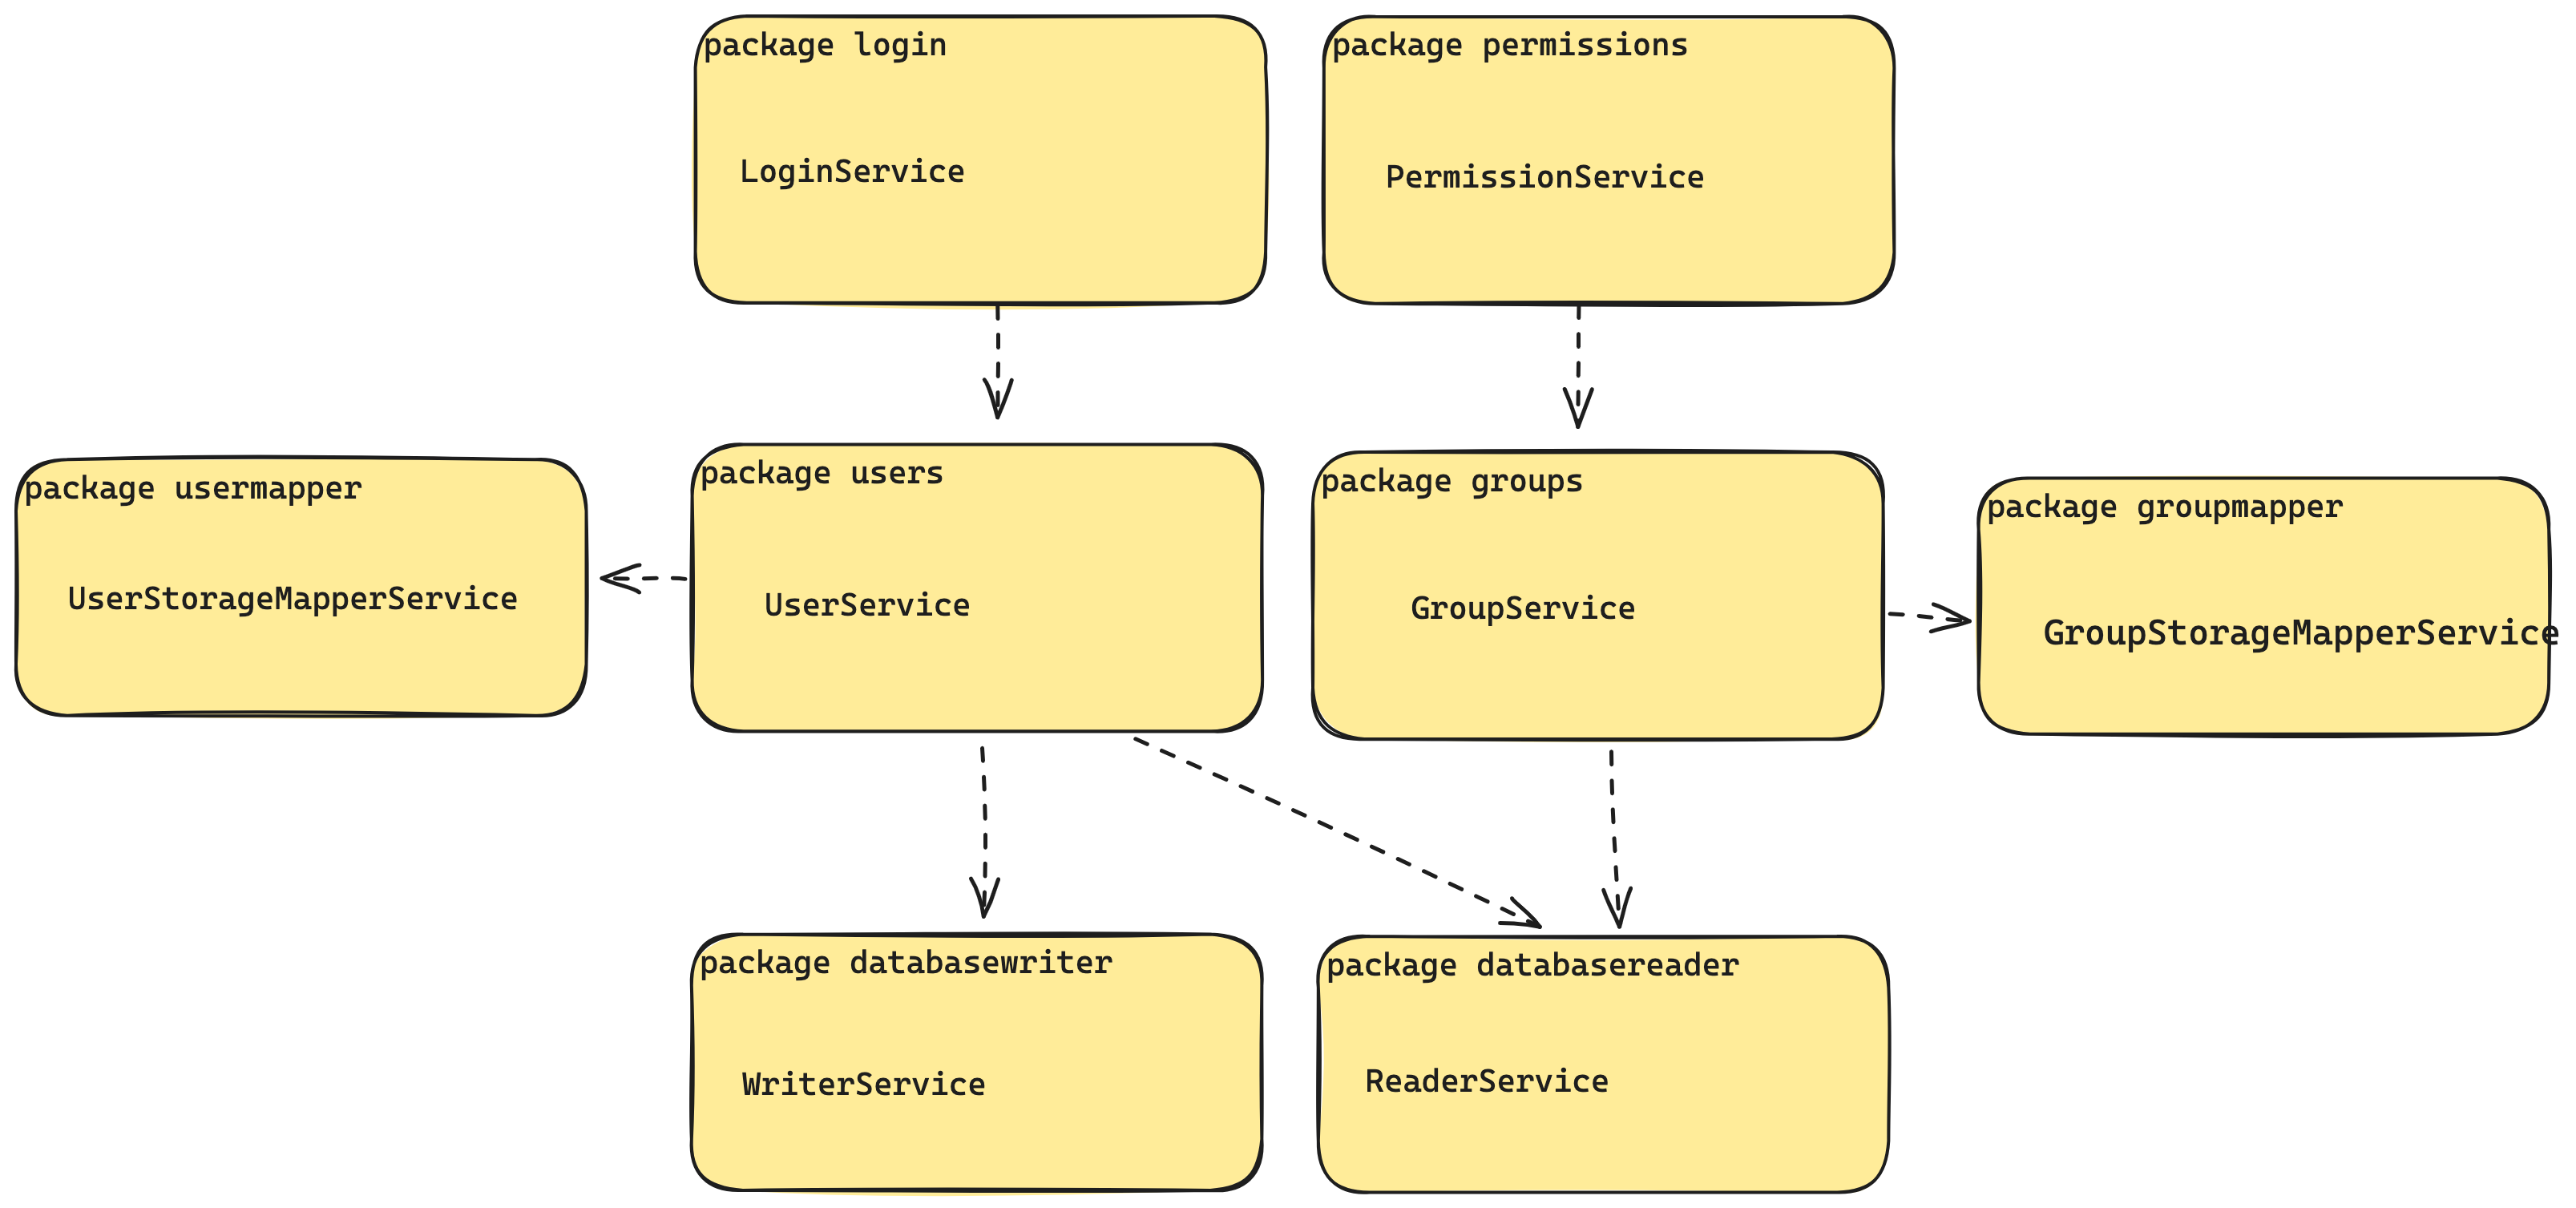
\includegraphics[scale=0.13]{img/good_deps}
    \caption{Sistemos pavyzdys su aiškią, vieną funkciją turinčiais paketais}
    \label{img:good_deps}
\end{figure}

Toks skirstymo būdas taip pat sprendžia ciklinių priklausomybių problemą - pavyzdžiui, įrankio, skirto spręsti ciklinių priklausomybių problemą,
kūrimo aprašas~\cite{CircularDependencies} teigia, kad ciklinių priklausomybių problemą galima spręsti laikantis trijų principų -
bendro panaudojimo, bendro keitimosi bei paleidimo ir pernaudojimo ekvivalentumo.
Šie principai yra išvesti iš bendro saryšio principo ir akcentuoja, kad kartu besikeičiančios klasės turėtų būti viename pakete.
Tokiu atveju ciklinių priklausomybių tikimybė sumažėja.

Šio šablono pritaikymas gali būti sudėtingesnis - norint išskaidyti didesnės apimties paketą į kelis mažesnius, gali būti
sudėtinga atskirti, koks grupavimas tinkamesnis.
Tačiau, nors šį principą sunkiau pritaikyti, jis gali padėti išspręsti ne tik didelio klasių skaičiaus pakete problemą,
bet ir prisidėti prie mažesnio priklausomybių skaičiaus, taip užtikrinant sistemos tvirtumą.

Išanalizavus galimus kodo skirstymo į paketus šablonus didelio klasių skaičiaus pakete skirstymui, galima teigti, kad tinkamesnis sprendimas šiai
problemai yra skirstymas pagal smulkų funkcionalumą.


\subsubsection{Skirtingų sąsajų implementacijų skirstymo šablonų analizė}
Skirtingų sąsajų implementacijų skirstymui buvo išskirti du šablonai - sąsajų ir implementacijų grupavimas bei
įgyvendinimų atskyrimas.
Naudojant sąsajų ir implementacijų grupavimą, lengva rasti reikalingas implementacijas, tačiau šis būdas
turi vieną trūkumą - pakete su dideliu klasių kiekiu bei keliomis skirtingomis sąsajomis sunku suprasti, kuri klasė kurią sąsają įgyvendina.

Naudojant įgyvendinimų atskyrimą, galima labai greitai rasti sąsajas bei galimus jos įgyvendinimus beveik netyrinėjant sistemos struktūros bei klasių kodo.
Šis šablonas taip pat užtikrina, kad paketas turi vieną aiškų funkcionalumą, todėl laikosi bendro sąryšio principo.

Išanalizavus galimus kodo skirstymo į paketus šablonus skirtingų sąsajų implementacijų skirstymui, galima teigti, kad tinkamesnis sprendimas šiai
problemai yra įgyvendinimų atskyrimas.

\subsubsection{Esybių pokyčių ir versijavimo skirstymo šablonų analizė}
Esybių versijavimo skirstymui buvo išskirtas skirtingų versijų grupavimo į paketus šablonas.
Toks skirstymo būdas leidžia išvengti kodo duplikacijos bei perteklinio klasių skaičiaus paketuose, bei užtikrina aiškią skirtingų versijų
atskirtį. Toks būdas gali praplėsti skirstymą pagal dalykinę sritį - skirstomos versijos gali atspindėti reikalingus
palaikyti besikeičiančius verslo reikalavimus.
